\section{Mechanical Design}

\subsection{Screw Feeder}
% TODO: FIX Citation and Picture
\begin{figure}[h]
\centering
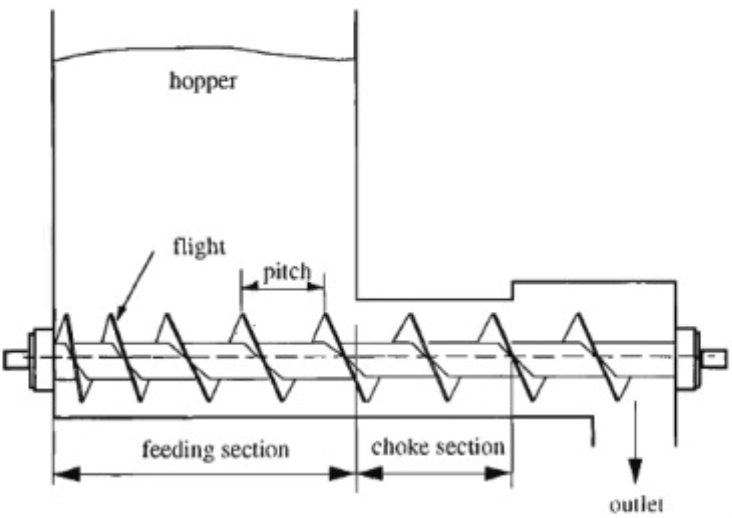
\includegraphics[width=6cm]{ch4/Screw_Feeder_Diagram.png} % replace with image path
\caption{Screw Feeder Diagram}
\label{fig:screw_feeder_diagram}
\end{figure}

% TODO: Update Citation
Figure \ref{fig:screw_feeder_diagram} shows the diagram of a screw feeder. Screw feeders are usually used in industrial fields like agriculture, chemicals, plastics, cements, poultry and food processing. According to \cite{Minglani_Sharma_Pandey_Dayal_Joshi_Subramaniam_2020}, screw feeders are specifically used to transport or move granular materials at a controlled rate like corn and wheat. It consists of a rotating screw and small feeding section or the hopper. Despite having big batches of a certain material, screw feeders can control the rate of which these materials are dispensed. With this concept, the group decided to utilize a screw feeder as the input mechanism for the system. This mechanism allows a controlled rate of coffee bean dispensing, which is a significant factor to avoid overcrowding in the rotating conveyor table causing the beans to jam. In addition, batches of coffee beans can be put at once instead of just adding a certain amount of beans at a time. 

\subsection{Rotating Conveyor Table}
\begin{figure}[h]
    \centering
    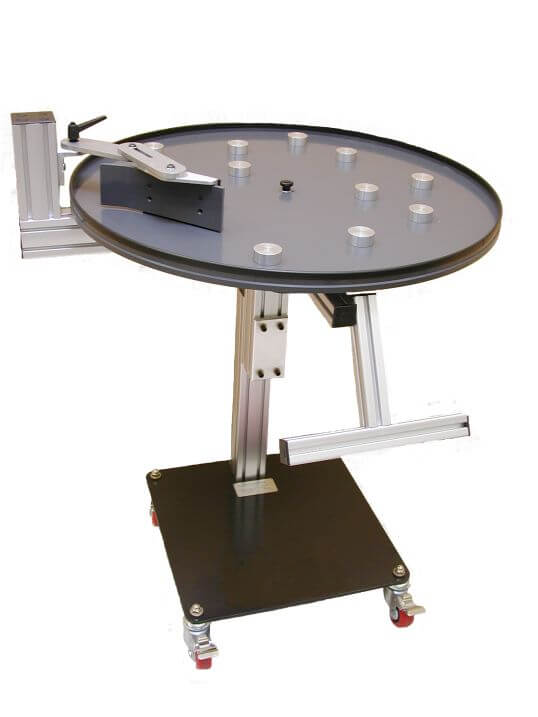
\includegraphics[width=6cm]{ch4/rotating_conveyor_table.jpg} % replace with image path
    \caption{Rotating Conveyor Table 3D Design, 32-inch Rotary Table Accumulator (RTA)}
    \label{fig:rotating_conveyor_table}
\end{figure}

After the inputted beans comes out from the screw feeder, the coffee beans would then be placed in the rotating conveyor table. According to the study of \cite{Dabek_Krot_Wodecki_Zimroz_Szrek_Zimroz_2022}. The conveyor table is used as a transportation systems for all forms of bulk materials to a certain machine or destination. The system utilizes the rotating conveyor table to have a controlled movement of coffee beans towards the first stage of the system. The improvised linearization system, consisting of metal guide rails and dividers ensures that beans align in a single path, reducing random movement, and improving the flow of the input beans. An infrared sensor would detect each bean as it passes, to control the movement of the bean preventing clogging and ensuring efficient operation. 

\subsection{Inspection Tray (1st Stage)}

\begin{figure}[h]
    \centering
    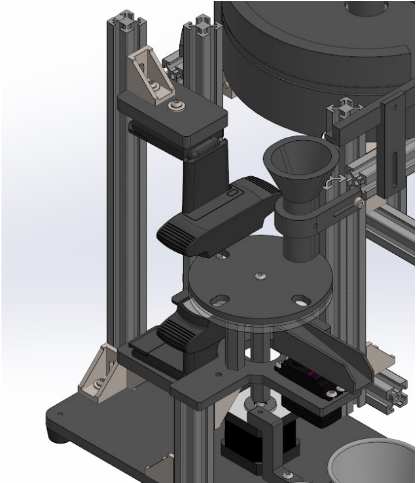
\includegraphics[width=6cm]{ch4/Inspection_Tray_3D_Design.png} % replace with image path
    \caption{Inspector Tray 3D Design}
    \label{fig:inspection_tray}
\end{figure}

The inspection tray serves as the platform for the machine vision based analysis of coffee beans. It is designed with 8 holes, allowing uniform placements and optimal camera positioning for the system. The system utilizes a two-layer structure: a stationary acrylic platform and a rotating 3D-printed platform with holes. The rotating mechanism sequentially positions each bean between two webcams, which captures and analyzes its physical characteristics from top and bottom perspective. This design captures both sides of the bean, ensuring a better classification of the bean. After inspection, the bean moves onto a slide, where it is either directed to the second stage for density analysis (Good) or sorted out as a defect.

\subsection{Density Sorter (2nd Stage)}

In measuring the density of the coffee bean there are a number ways this can be done, one way is by measuring the bulk density of the batch. This is done by measuring the mass of a batch then dividing it to a fixed volume. The more appropriate method for measuring the density of the coffee bean is called “free settle” density or free-flow density. This is defined as the ratio of the mass of the coffee beans to the volume they occupy after being allowed to flow freely into a container. It is expressed in grams per liter or kilograms per cubic meter. 

\section{Embedded Systems}

\subsection{Microcontroller}

\begin{figure}[H]
    \centering
    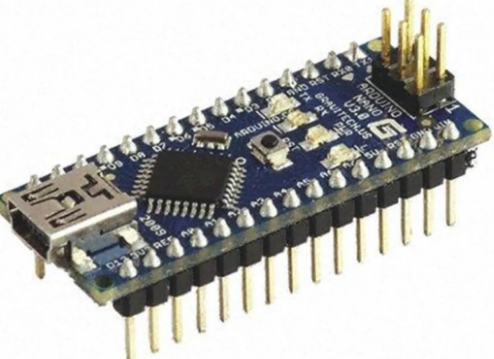
\includegraphics[width=6cm]{ch4/Arduino_Nano_Microcontroller.png} % replace with image path
    \caption{Arduino Nano Microcontroller}
    \label{fig:arduino_nano}
\end{figure}

Since the system is composed of two stages of sorting: defect sorting through computer vision and density-based analysis–the group decided to utilize two Arduino Nano microcontrollers to modularize the control process. The first Arduino Nano microcontroller is tasked to handle the computer vision-based defect sorting through serial communication with OpenCv operating in Python. In addition, it handles the operation of defect sorting consisting of a stepper motor for the rotation of the inspection tray and a servo motor for the slider, which directs the beans to the designated bin (defect or good bin). On the other hand, the second Arduino Nano microcontroller manages the density-based analysis and sorting, which consists of another stepper motor to direct the beans to its respective bin (dense and less-dense bin), the precision scale which is interfaced through RS232, and the top feeder where the input beans are poured. The use of separate Arduino microcontrollers is advantageous when it comes to the computer vision-based sorting of beans. This is because serial communication is much faster when code complexity is significantly reduced. With this, a designated microcontroller handles the computer vision part and two-way serial communication between the microcontroller and the computer vision algorithm running in Python. Most importantly, the use of two microcontrollers allowed the system to not rely solely on a sequential approach. This means that the two stages of sorting are not relying on the timing of each other, allowing the inspection tray and the top feeder to operate independently. Thus, resulting in a much faster and efficient sorting process. 

\subsection{Sensors}

\begin{figure}[H]
    \centering
    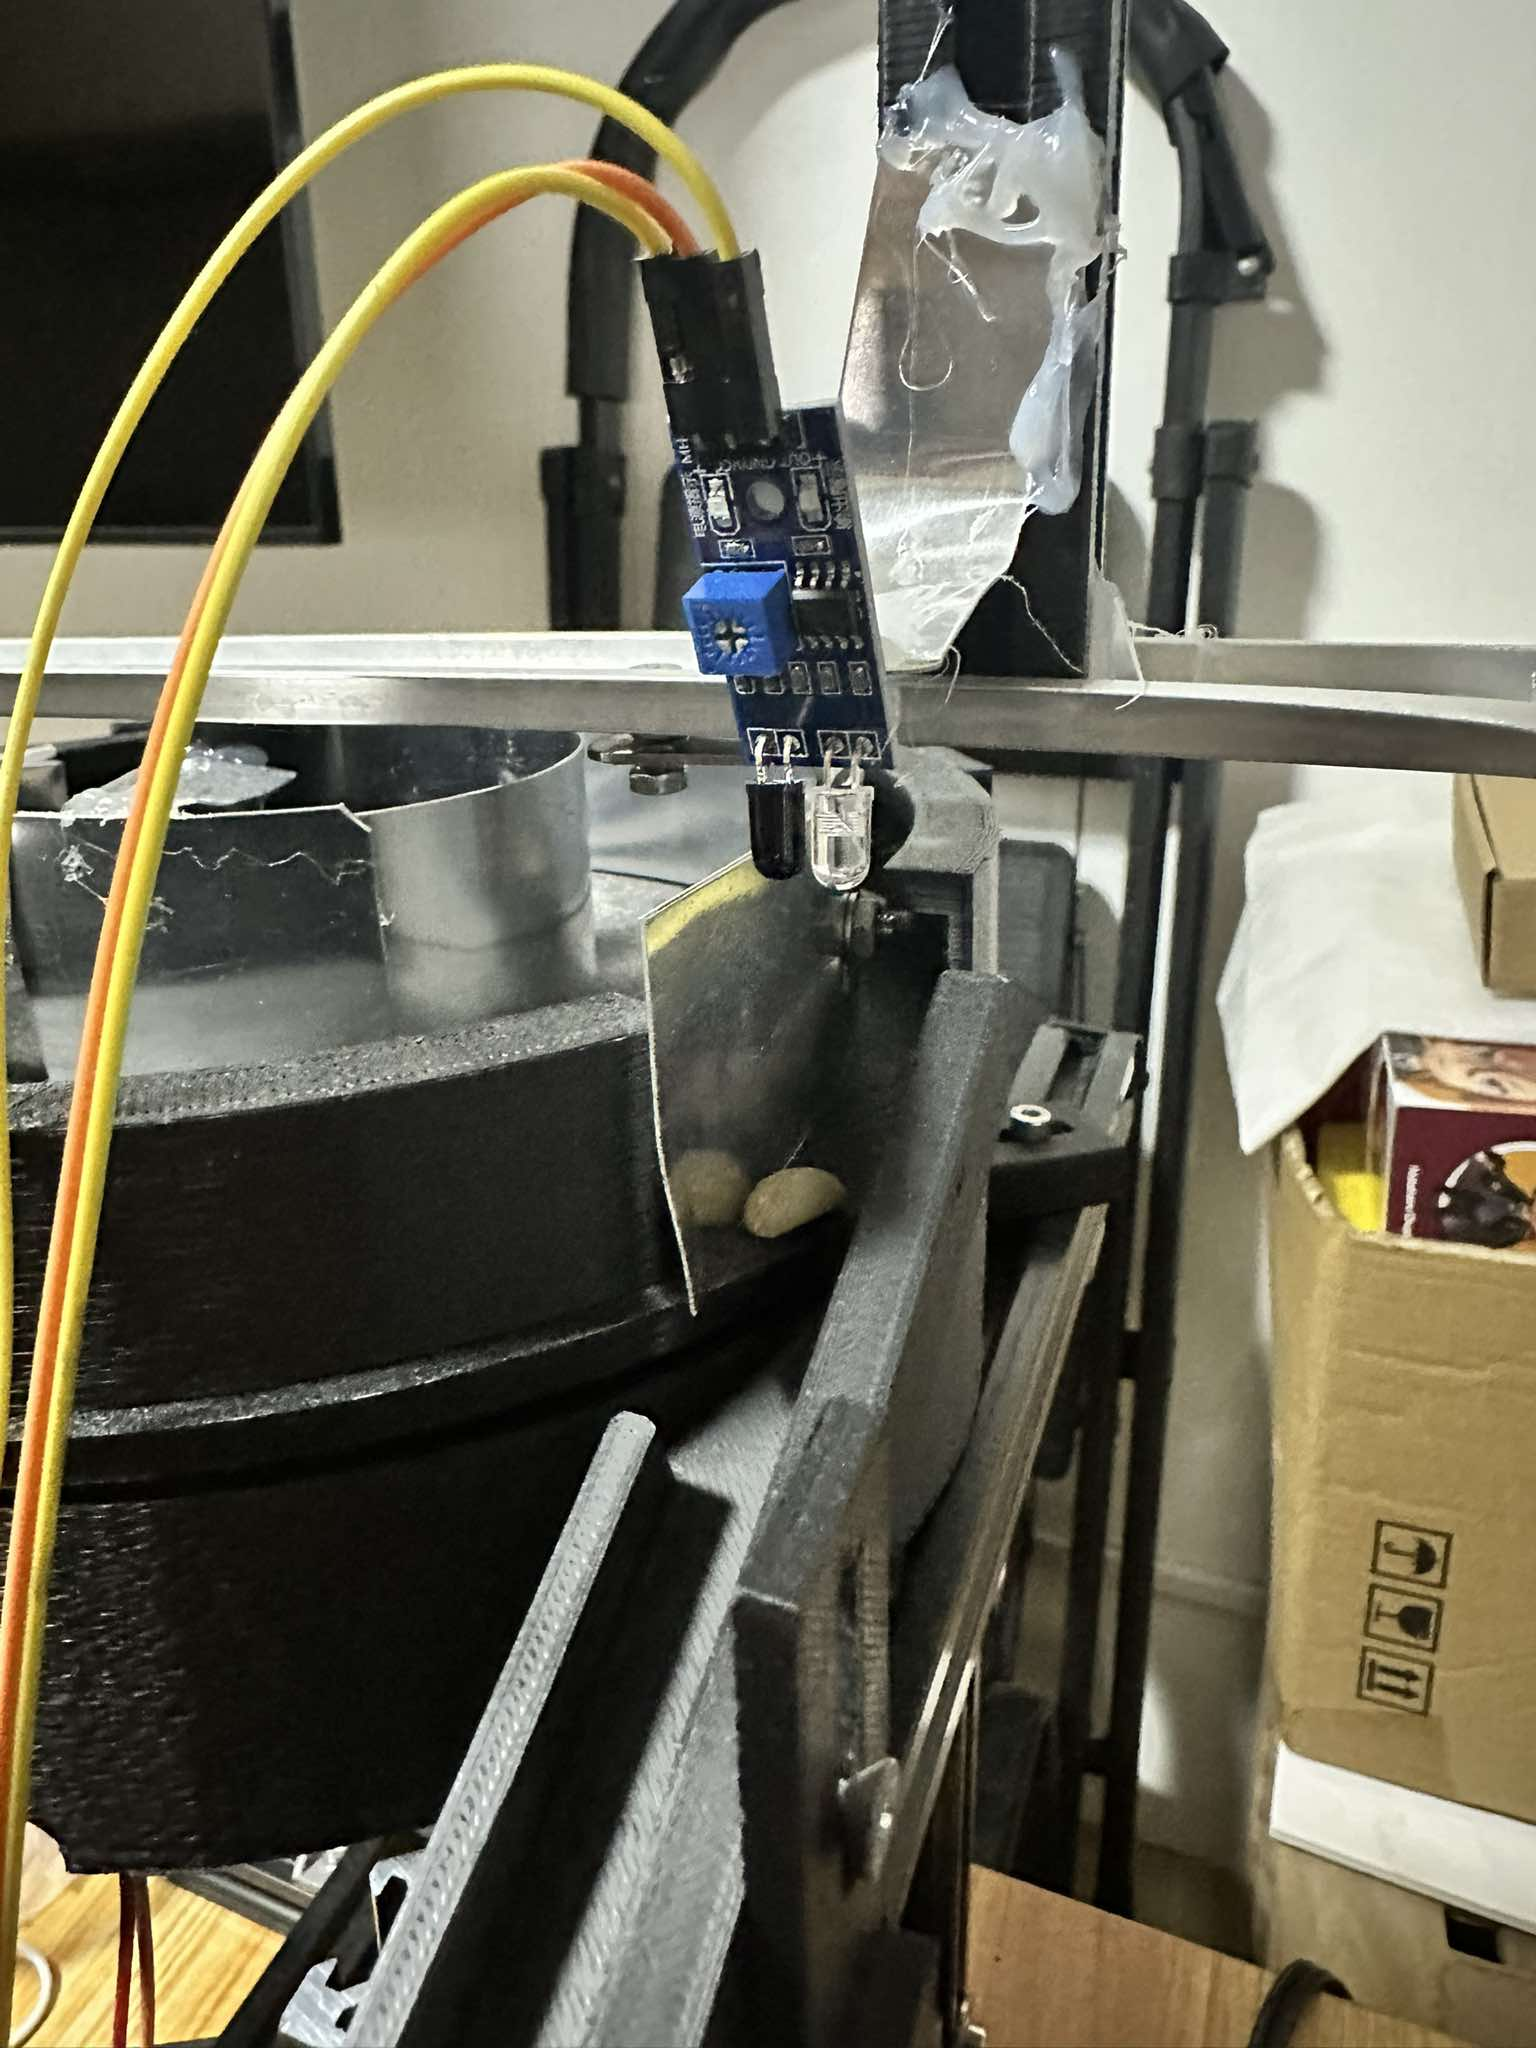
\includegraphics[width=6cm]{ch4/Infrared_Sensor.jpg} % replace with image path
    \caption{Infrared Sensor}
    \label{fig:infrared_sensor}
\end{figure}

To ensure that the beans are falling in a one-by-one manner onto the inspection tray, the group placed an IR sensor at the edge of the top feeder. This IR sensor triggers the DC motor that runs the feeder to stop, and runs small steps until the bean is dropped. The addition of the IR sensor at the edge of the feeder allows the motor to run continuously until another bean is detected. With this, the waiting time for the next bean at the inspection tray is significantly lessened. 

\begin{figure}[H]
    \centering
    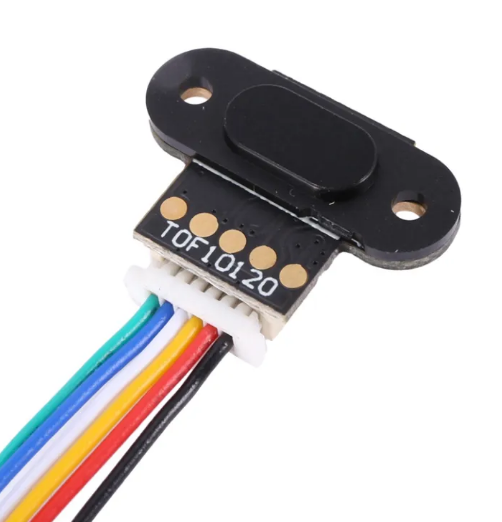
\includegraphics[width=6cm]{ch4/TOF10120.png} % replace with image path
    \caption{TOF10120}
    \label{fig:tof10120}
\end{figure}

TOF10120 or Time of Flight sensor is utilized in the system due to its high precision, non-contact measurement capability. This sensor is used to estimate the volume of each bean, which is essential for computing the density. In the second stage of sorting, where beans are classified based on density, the sensor plays a crucial role in determining the approximate volume of each bean by measuring its height or dimensions as it passes through the system.

\subsection{Motor control}

\begin{figure}[H]
    \centering
    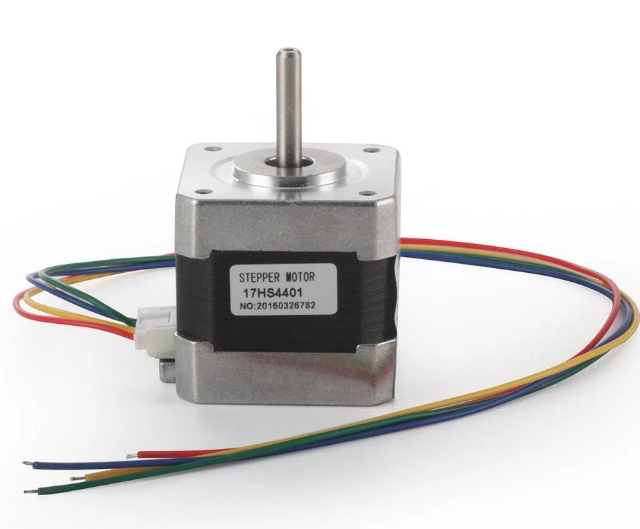
\includegraphics[width=6cm]{ch4/12V_NEMA_17_Stepper_Motor.png} % replace with image path
    \caption{12V NEMA 17 Stepper Motor}
    \label{fig:stepper_motor}
\end{figure}

Two NEMA 17 12V stepper motors, paired with L298N motor drivers were used to control the movement of the inspection tray in the first stage and the density-based sorting mechanisms in the second stage. In these mechanisms, the group decided to use stepper motors to ensure precise and accurate movements. Precise and accurate movements are needed for the inspection tray to make sure every movement of the hole is perfectly aligned to the camera. Thus, allowing a more uniform and consistent angle for each bean to be inspected through the computer vision. In addition, NEMA 17 stepper motors were the best choice for these mechanisms due to its high torque, which is essential because it will be moving weighted objects. 

\begin{figure}[H]
    \centering
    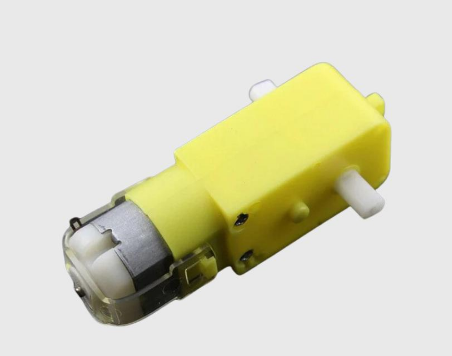
\includegraphics[width=6cm]{ch4/6V_DC_Motor.png} % replace with image path
    \caption{6V DC Motor}
    \label{fig:6v_dc_motor}
\end{figure}

For the rotating conveyor table (top feeder), where the beans are initially poured, a 6V DC motor is used. The group decided to use this motor due to its high RPM, which is needed for a fast rotation of the rotating conveyor table. The speed of the feeder is regulated to prevent clogging and ensure that the beans are evenly spaced before they enter the inspection tray. The motor speed is fine-tuned through pulse-width modulation (PWM) to synchronize with the stepper motor-driven inspection tray, ensuring a steady input without overwhelming the system.

\begin{figure}[H]
    \centering
    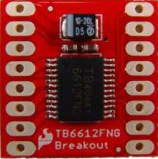
\includegraphics[width=6cm]{ch4/TB6612FNG_Motor_Driver.png} % replace with image path
    \caption{TB6612FNG Motor Driver}
    \label{fig:motor_driver}
\end{figure}

To drive the 6V DC motor, the group utilized TB6612FNG, a motor driver module. This module also allowed PWM control for the motor, which is essential for reducing the speed of the motor when needed. 

\subsection{Operating Voltage}

\begin{figure}[H]
    \centering
    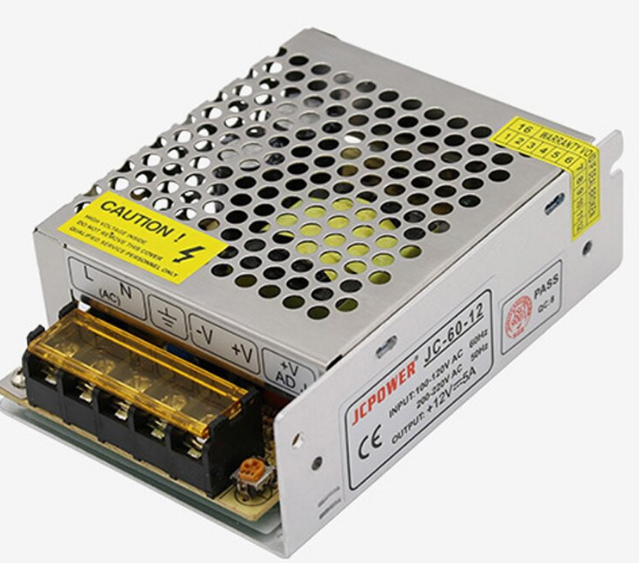
\includegraphics[width=6cm]{ch4/12V_Power_Supply.png} % replace with image path
    \caption{12V Power Supply}
    \label{fig:12v_power_supply}
\end{figure}

The main power supply comes from a 12V external power supply, which provides enough voltage for all the components and keeps the voltage from dropping and interfering with system performance. The Arduino microcontroller is powered via its VIN pin, so it can function without the need for a USB connection and maintains a stable 5V logic output for sensor and actuator control. The NEMA 17 stepper motors that operate the inspection tray and density sorter are directly powered from the 12V supply and fed into L298N motor drivers to adjust voltage and monitor current flow. Operating these motors at 12V provides best torque output, which is vital in ensuring consistent movement during the sorting process.

\begin{figure}[H]
    \centering
    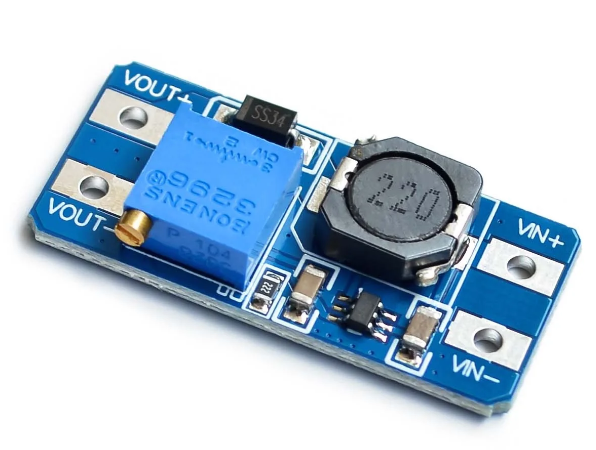
\includegraphics[width=6cm]{ch4/MT3608_Step-Up_Module.png} % replace with image path
    \caption{MT3608 Step-Up Module}
    \label{fig:mt3608}
\end{figure}

For the top feeder mechanism, a step-up module is needed to supply the sufficient voltage needed for the motor–6V. From the 5V output of the Arduino, the step-up module will be utilized to convert it into 6V.

\section{Computer Vision System}
% TODO: Write content
\subsection{Image Processing}

\begin{figure}[H]
    \centering
    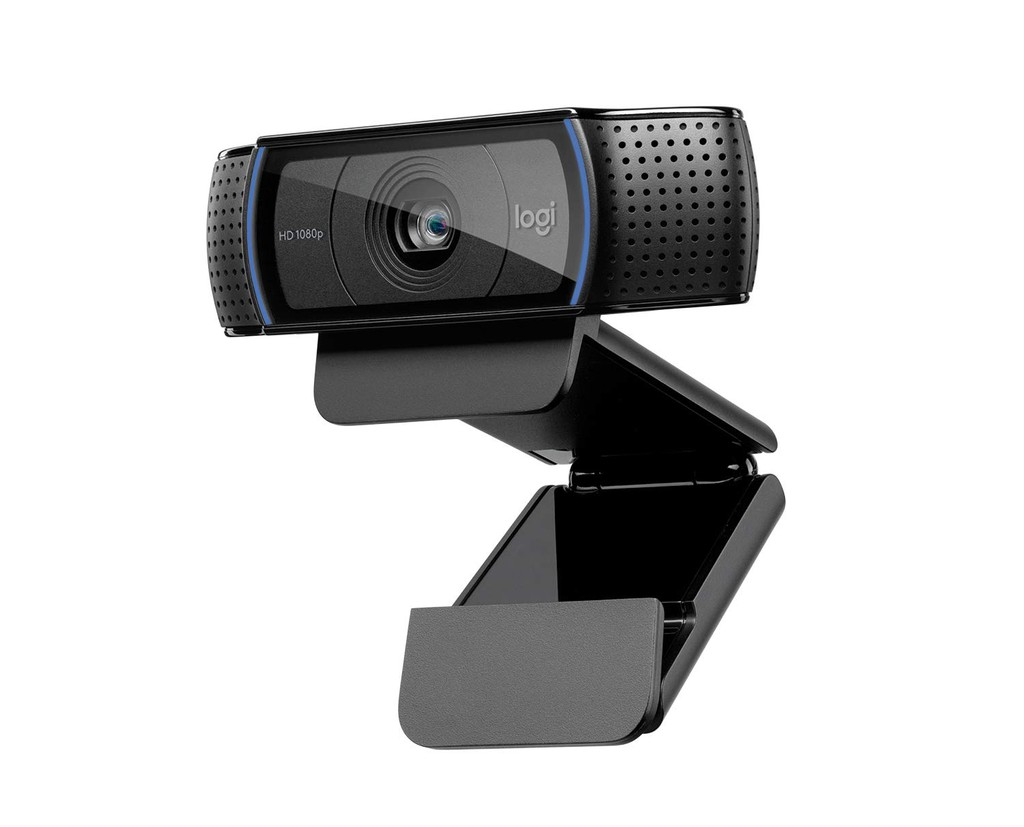
\includegraphics[width=6cm]{ch4/c920_cam.png} % replace with image path
    \caption{C920 Camera}
    \label{fig:c920_camera}
\end{figure}

The system requires clear images of the coffee beans for accurate processing by the detection and classification models. Two C920 cameras will be used to capture images from opposite sides of each bean—one positioned on top and the other at the bottom. The captured images will then be processed within the laptop using the detection and classification models to identify and categorize the beans.

\subsection{Object Detection and Classification Models}

The object detection model identifies and isolates the coffee beans from the background. For this task, different models were explored:

\begin{enumerate}
	\item \textbf{RF-DETR}
	 
	A transformer-based object detection model that eliminates the need for anchor boxes, improving small object detection.

	\item \textbf{YOLOv11}
	
	A CNN-based YOLO variant that incorporates the C3k2 block, SPPF, and C2PSA components to enhance feature extraction and detection accuracy.

	\item \textbf{YOLOv12}
	
	The latest YOLO version and attention-centric model that integrates transformer-based components to enhance performance while maintaining real-time efficiency.
\end{enumerate}

\subsection{Object Classification Models}
Following detection, each identified coffee bean was cropped and classified based on its defect type. The classification models used included:

\begin{enumerate}
	\item \textbf{EfficientNetV2}
	 
	A convolutional neural network (CNN) designed for high efficiency and accuracy, balancing computational cost and performance.
	
	\item \textbf{YOLOv8}
	
	A lightweight yet highly accurate model that supports both object detection and classification, making it suitable for real-time applications.

	\item \textbf{YOLOv11}
	
	A classification-specific adaptation of YOLOv11, leveraging enhanced feature extraction techniques for defect recognition.
	
	\item \textbf{YOLOv12}
	
	A classification variant of YOLOv12, incorporating advanced attention mechanisms to improve accuracy.
\end{enumerate}

\section{Serial Communication}

Serial communication is used for sensors and motors for arduino due to the simplicity, reliability and efficient transfer of data between different devices. The precision scale uses a RS232 and a MAX TTL converter to send the data from the precision to the arduino to get the weight values of each green coffee bean. To sort out the good from defective beans the system utilizes a servo motor. The data from python is received by the arduino through serial communication. The python side is responsible for the decision and defect classification while the arduino is responsible for controlling the servo motor.  

\section{Graphical User Interface (GUI)}

% TODO: Update design to consider new features (Tracking which defects are present, density details, the recommendation based on thresholding, the speed of system, runtime, accessibility etc.)
\begin{figure}[h]
    \centering
    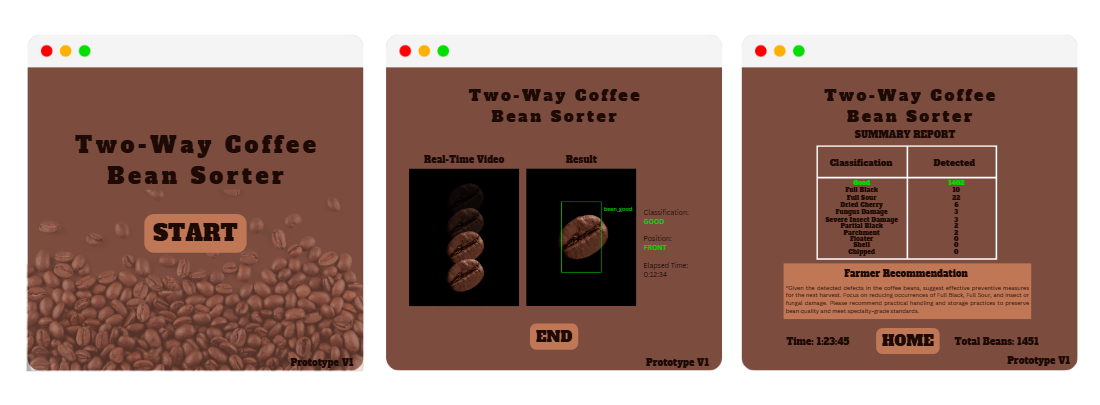
\includegraphics[width=12cm]{ch5/GUI.png} % replace with image path
    \caption{Graphical User Interface}
    \label{fig:gui}
\end{figure}

The proposed system would be integrating a graphical user interface developed using PyGui and ChatGPT API. The GUI would serve as the control center platform for the system. This would provide real-time feedback and insights for users. As shown in Figure 8, a concept of how the GUI would interact with the system would be a start button, once the button is executed the system would then be expecting inputs and start sorting. There would be real-time feedback during the sorting process, then some visual markers to indicate their classification, and an elapsed time so the user would be aware of the time of the sorting process. Once the system is done, the user can click the end button and the summary report would generate in an orderly manner, providing tables of classification that was detected through the process. In the bottom part of the GUI, ChatGPT API would be integrated and would offer recommendations based on the detected quality and classification of the coffee beans. 

\section{Density Analysis}
The density analysis works by using a precision scale to measure the mass of the bean. To get the data from the precision scale, serial communication is used from the scale to an arduino nano. This is done by using a RS232 with a Max TTL converter for the arduino to read the data from the precision scale. To sort out the good from defective beans the system utilizes a servo motor for the density sorting mechanism. The servo motor is used to sort the dense from the less dense beans. The sorting mechanism developed consists of gears and cross-shaped modules to properly capture the beans and properly sort them out. 

\section{Technical Standards}

\subsection{Hardware}
In the design and development of the system, the group incorporated and followed a series of technical standards. One of which is ISO 12100:2010 – Safety of Machinery, where general principles for risk assessment and reduction are discussed. Thus, the system is designed, while keeping in mind the hazards associated with moving parts, making sure that all moving parts in the system do not need to be touched for operations. An emergency stop is also integrated into the system to stop all the moving parts in case of undesirable incidents \cite{International_Organization_for_Standardization_2010}. 

On top of this, ISO 14121-1 – Risk Assessment for Machinery was also followed to further assess the potential risks throughout the system. The standard includes identifying and quantifying hazards such as electrical short circuits, faulty wirings, and motor overheating \cite{International_Organization_for_Standardization_2007}. With this, the system included protective enclosures for the electrical wirings, proper grounding of the circuits, and controlled motor actuation. More specifically, for motors, it was made sure that the design has sufficient voltage and ampere to power the different kinds of motors used with the use of L298N, and MT3608 modules. These are the main components for adjusting motor speeds dynamically during the sorting process.

Lastly, ISO 30071-1 was standard used to provide sufficient lighting during data collection, and real time bean inspection during sorting process. This standard helps ensure consistent and non-glare lighting conditions, which are essential for the machine vision cameras to accurately capture bean features \cite{International_Organization_for_Standardization_2019}. Uniform illumination improves the reliability of image classification by reducing shadow artifacts and reflections, thereby enhancing overall detection performance.

\subsection{Software}

For the software side of the system, the first applicable standard is ISO/IEC 25024 – Systems and Software Engineering – Measurement of Data Quality, which offers a systematic method for measuring the quality of datasets utilized in information systems \cite{International_Organization_for_Standardization_2015}. This standard was used during the dataset gathering and training for the different coffee bean defects like black, sour, insect damage, fungus damage, broken, floaters, and dried cherry. Practically, this included pre-processing the image data to eliminate noise, balance class distribution, and verify ground truth labels. 

Lastly, ISO/IEC 23053 – Framework for Artificial Intelligence (AI) offers a reference architecture to build and integrate machine learning building blocks \cite{International_Organization_for_Standardization_2022}. This standard was highly applicable in determining the design of the machine vision module, where a pre-trained deep learning model is utilized for the classification of bean defects. This standard provides guidelines on best practice for the overall machine learning cycle, ranging from data acquisition, feature extraction, and model training through to model evaluation, deployment, and monitoring. 

\subsection{Green Coffee Bean Sorting}

For sorting green coffee beans, Specialty Coffee Association of America (SCAA) Standards for Green Coffee Bean Sorting was incorporated to maintain conformity. The standards set the definition for the classification of primary and secondary defects (i.e., black, sour, insect-damaged, broken, and floater beans) and sets the maximum allowable defect counts for specialty-grade coffee. The SCAA standards were applied to mark the training set of the machine vision model and also to set up the thresholds of defect classification, so visually defective beans can be correctly classified and rejected. Also, the sorting mechanism based on density points towards SCAA bean weight and volume guidelines using a precision scale and ToF sensor to sort beans based on within-acceptability density limits.

On the other hand, the system also adheres to PNS/BAFS 341:2022, the Philippine National Standard for Agricultural Machinery – Coffee Green Bean Grader – Specifications and Methods of Test \cite{Bureau_of_Agriculture_and_Fisheries_Standards_2022}. It sets local criteria for testing coffee grading equipment on performance, safety, construction aspects, and methods of test. For the purposes of this research, PNS/BAFS 341:2022 is used as a reference for the design of the sorting mechanism, specifically in terms of the materials used in construction, handling of beans, and the efficiency with which the mechanical and electronic subsystems segregate. It also guides the testing procedure employed to verify sorting precision, capacity, and rates of misclassification under test conditions. 
